\documentclass[12pt,xcolor=dvipsnames]{beamer}
\usepackage{amsmath,amssymb,amsfonts}
\usepackage{dcolumn}
\usepackage{booktabs}
\usepackage{lmodern}

\usepackage[T1]{fontenc}
% ,linkcolor=,urlcolor=links}
\usepackage{hyperref}
\hypersetup{colorlinks}

\usetheme{IS2012Tutorial}
%%% load AMS-Latex Package
\usepackage{amsmath,amsfonts}
% \usepackage{amsthm}
\usepackage{amssymb,amsopn}
\usepackage{bm} % bold symbol

% define fonts
\newcommand{\vct}[1]{\boldsymbol{#1}} % vector
\newcommand{\mat}[1]{\boldsymbol{#1}} % matrix
\newcommand{\seq}[1]{\boldsymbol{#1}} % sequence

\newcommand{\set}[1]{\mathcal{#1}} % set

%%%% Special math symbols
\newcommand{\field}[1]{\mathbb{#1}}
\newcommand{\R}{\field{R}} % real domain
\newcommand{\C}{\field{C}} % complex domain
\newcommand{\F}{\field{F}} % functional domain
%\newcommand{\T}{^{\top}\!\!} % transpose
\newcommand{\T}{^{\textrm T}} % transpose
\newcommand{\TN}{^{-\textrm T}} % transpose
\DeclareMathOperator{\tr}{Tr}
\DeclareMathOperator{\diag}{diag}
\DeclareMathOperator{\tovec}{vec}

%%% define constant
\newcommand{\cst}[1]{\mathsf{#1}}

%% operator in linear algebra, functional analysis
\newcommand{\inner}[2]{#1\cdot #2}
\newcommand{\norm}[1]{\left\|#1\right\|}
\newcommand{\twonorm}[1]{\|#1\|_2^2}
% operator in functios, maps such as M: domain1 --> domain 2
\newcommand{\Map}[1]{\mathcal{#1}}

% operator in probability: expectation, covariance,
\newcommand{\ProbOpr}[1]{\mathbb{#1}}
% independence
\newcommand\independent{\protect\mathpalette{\protect\independenT}{\perp}}
\def\independenT#1#2{\mathrel{\rlap{$#1#2$}\mkern2mu{#1#2}}}
% conditional independence
\newcommand{\cind}[3]{{#1} \independent{#2}\,|\,#3}
% conditional expectation
\newcommand{\cndexp}[2]{\ProbOpr{E}\,[ #1\,|\,#2\,]}

% operator in optimization
\DeclareMathOperator*{\argmax}{arg\,max\:}
\DeclareMathOperator*{\argmin}{arg\,min\:}
\newcommand{\todo}[1]{{\color{red}#1}}

% Gaussian distribution
\newcommand{\gauss}[3]{\mathcal{N}(#1|#2,#3)}

% environment
\newtheorem{thm}{Theorem}

\newcommand{\eat}[1]{}

%
\newcommand{\src}{{\color{blue} \mathcal{S}}}
\newcommand{\tgt}{{\color{red} \mathcal{T}}}



%%%% Other commands to make presentation consistent
\newcommand{\heading}[1]{{\color{red}\textbf{#1}}}
\newcommand{\stress}[1]{{\color{ForestGreen}\textbf{\emph{#1}}}}
\newcommand{\nb}[1]{{\scriptsize \emph{{\color{RoyalPurple}N.B.\ }}\color{Brown}#1}}
% for url to work
\definecolor{links}{HTML}{2A1B81}

%%% For prettier tables
\newlength{\colA}
\newcommand{\aln}[3]{\makebox[#1][#2]{#3}}
\newcolumntype{d}[1]{D{.}{.}{#1}}

% to get references in an easy way, from one BiBTeX file
\usepackage{bibentry}
\def\newblock{\hskip .11em plus .33em minus .07em}
\setbeamertemplate{frametitle continuation}{}
\setbeamertemplate{bibliography item}{\insertbiblabel}

% \usepackage[contents={DRAFT},scale=5]{background}
% \setbeamertemplate{background}{\BgMaterial}

%\usepackage{draftwatermark}
%\SetWatermarkText{DRAFT}
%\SetWatermarkScale{0.4}
%\setbeamercolor{background canvas}{bg=}%transparent canvas

\mode<presentation>

% max figure size is 108 x 72 mm

\author{Florian Metze, Samuel Thomas, \\
  Bhuvana Ramabhadran, and Brian Kingsbury}
\title{{\color{Maroon} Pushing the frontiers of speech processing --- What does it take to tackle new languages and domains?}}
\institute{Carnegie Mellon University and IBM}
\date{\today}

\sloppy

\begin{document}

\section{Title}

\begin{frame}
  \titlepage
\end{frame}

\begin{frame}{For the most recent version of this presentation}{}
  \centering
  \url{https://github.com/bedk/IS2016-Tutorial/blob/master/main.pdf}
\end{frame}

\begin{frame}
  \frametitle{Florian Metze}
  \begin{columns}[T]
    \column{2in}
    \begin{itemize}
    \item Associate Research Professor at Carnegie Mellon University (LTI/SCS)
    \item End-to-end Speech Recognition
    \item Articulatory Features for Speech Recognition
    \item Multi-media Analysis
    \item \texttt{fmetze@cs.cmu.edu}
    \end{itemize}
    \column{2in}
    \framebox{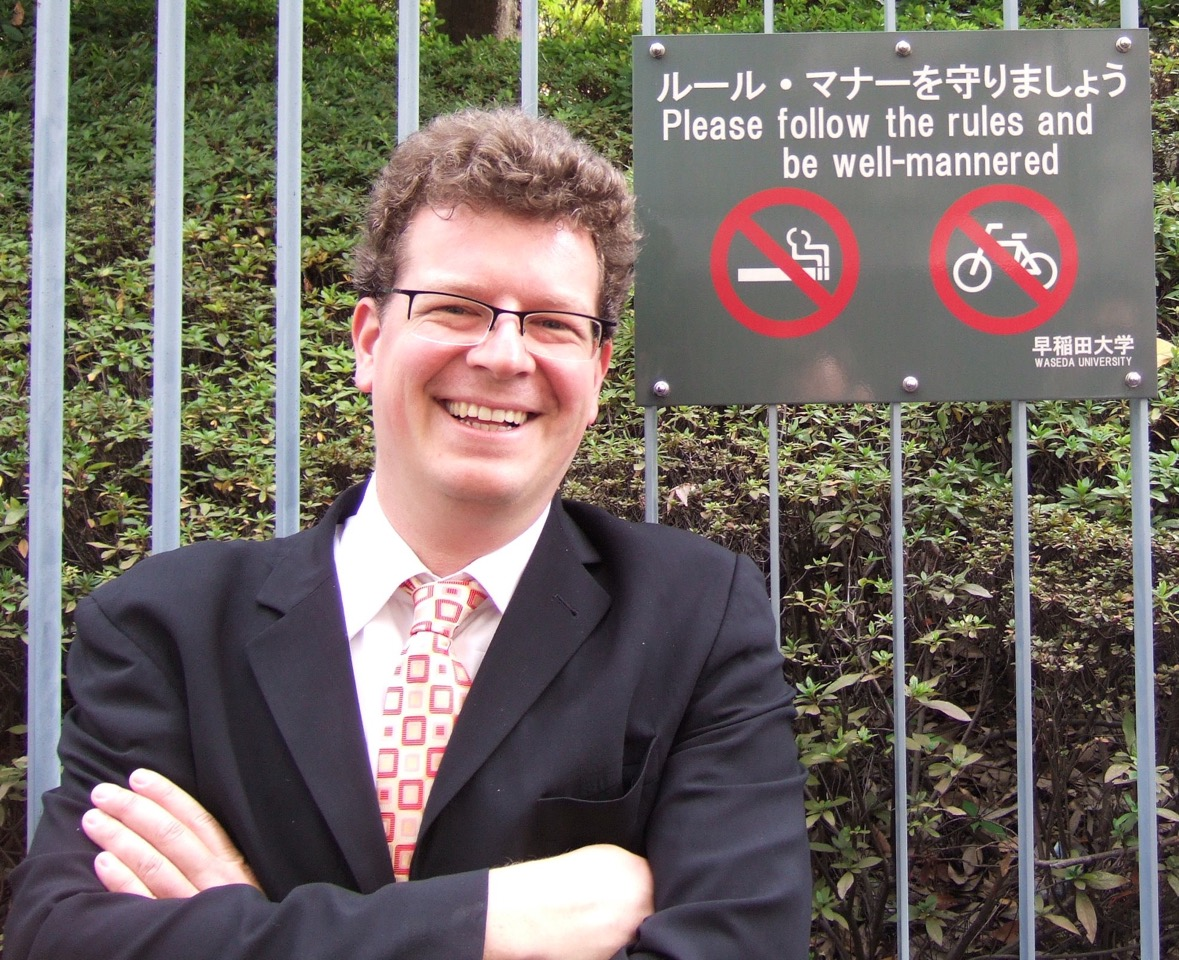
\includegraphics[width=2in]{figures/Florian}}
  \end{columns}
\end{frame}

\begin{frame}
  \frametitle{Samuel Thomas}
  \begin{columns}[T]
    \column{2in}
    \begin{itemize}
    \item Researcher in the IBM Watson Group
    \item Automatic Speech Recognition
    \item Feature Engineering and Acoustic Modeling
    \item \texttt{sthomas@us.ibm.com}
    \end{itemize}
    \column{2in}
    \framebox{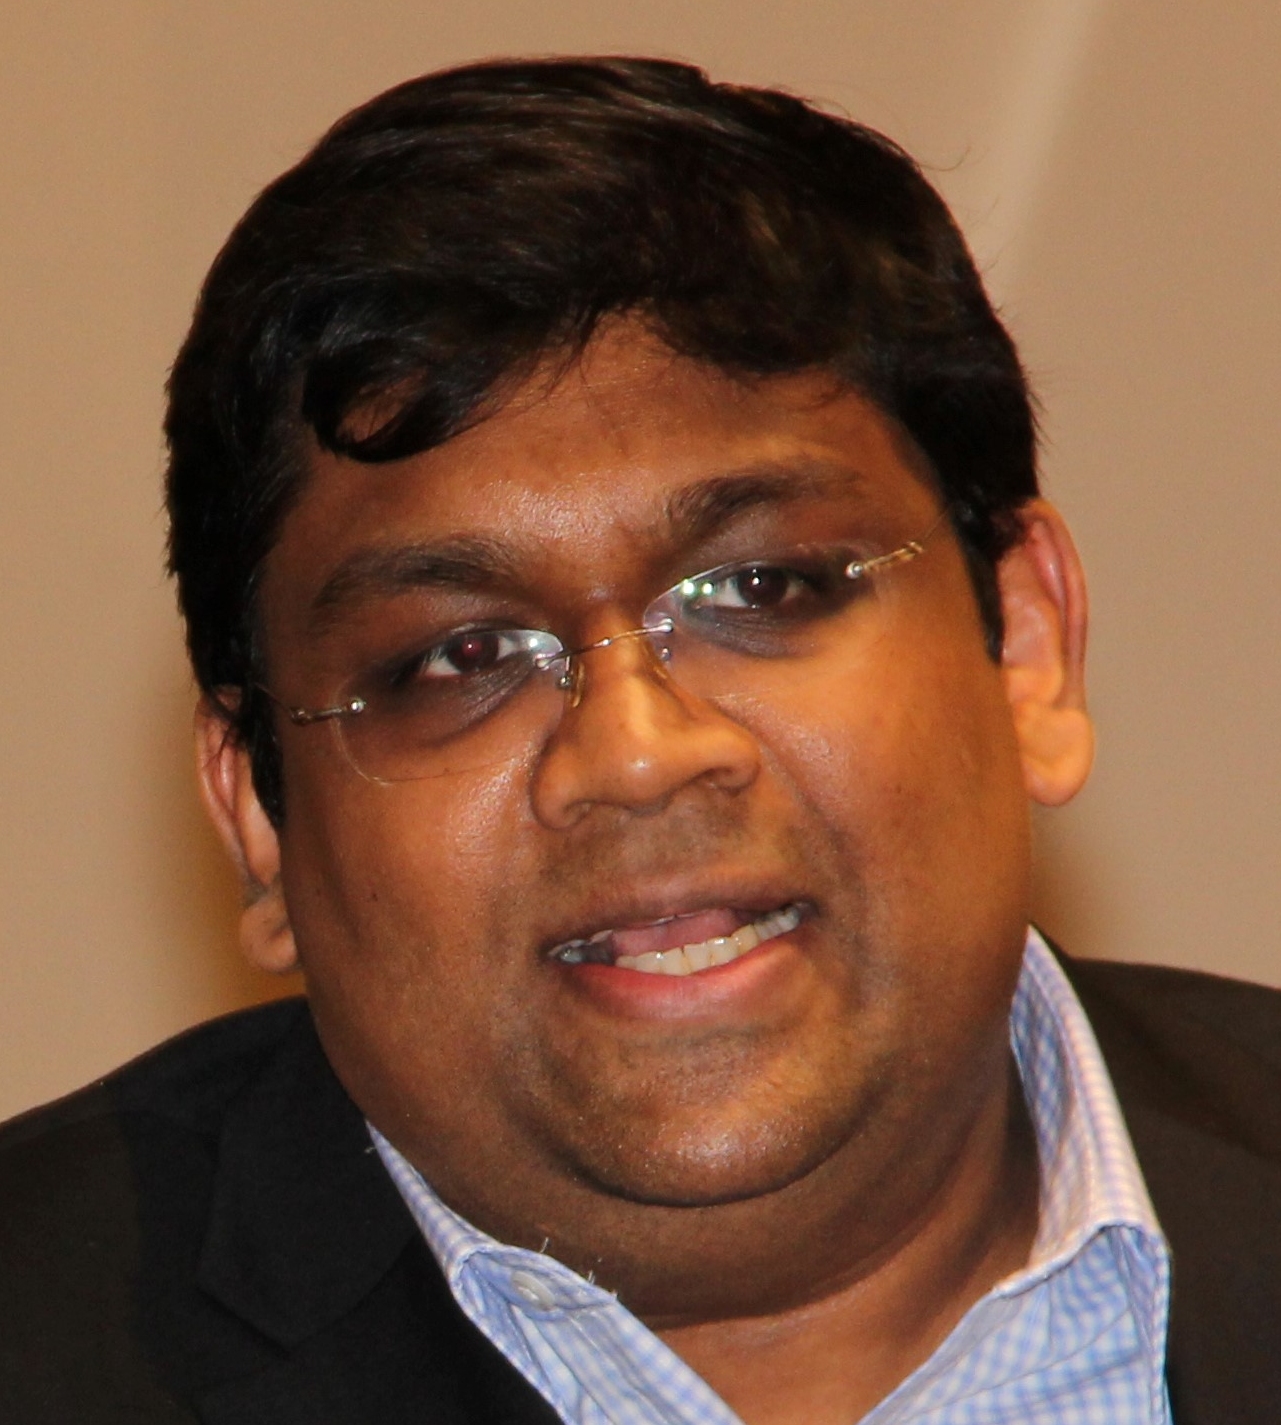
\includegraphics[width=1.5in]{figures/Sam}}
  \end{columns}
\end{frame}

\begin{frame}
  \frametitle{Bhuvana Ramabhadran}
  \begin{columns}[T]
    \column{2in}
    \begin{itemize}
    \item Research Manager in the IBM Watson Group
    \item Automatic Speech Recognition
    \item Deep Learning for Acoustic and Language Modeling
    \item Keyword Search
    \item \texttt{bhuvana@us.ibm.com}
    \end{itemize}
    \column{2in}
    \framebox{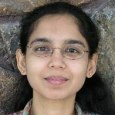
\includegraphics[width=1in]{figures/Bhuvana}}
  \end{columns}
\end{frame}

\begin{frame}
  \frametitle{Brian Kingsbury}
  \begin{columns}[T]
    \column{2in}
    \begin{itemize}
    \item Research Scientist in the IBM Watson Group
    \item Deep Learning
    \item Automatic Speech Recognition
    \item Keyword Search
    \item \texttt{bedk@us.ibm.com}
    \end{itemize}
    \column{2in}
    \framebox{\includegraphics[width=2in]{figures/Brian}}
  \end{columns}
\end{frame}


\begin{frame}
  \frametitle{Outline (3 hours)}
  \begin{enumerate}
  \item Introduction
  \item Tackling a New Language
  \item Tackling a New Domain
  %\item Lessons Learnt with Current Neural Network Technologies
  \item Research Topics, Challenges, and New Ideas
  \item End-to-End Systems
  \item Virtual Machines and Tools
  \item Conclusions
  \end{enumerate}
\end{frame}

\section{Introduction}
\begin{frame}
  \begin{center}
    {\color{Maroon}\Huge Introduction}
  \end{center}
\end{frame}

%% put section outline here


\section{New Languages}
\begin{frame}
  \begin{center}
    {\color{Maroon}\Huge Tackling New Languages}
  \end{center}
\end{frame}

\begin{frame}{Tackling New Languages}{Outline}
  \begin{enumerate}
  \item IARPA Babel
  \item Audio Keyword Search
  \item What Language Characteristics Matter?
  \item A Recipe for a New Language
  \end{enumerate}
\end{frame}

\begin{frame}{The IARPA Babel Program}{}
  \Large{``\ldots to \alert{rapidly develop} speech recognition
    capability for keyword search in a previously unstudied
    language, working with speech recorded in a variety of
    conditions with limited amounts of transcription.''}\par
\end{frame}

\begin{frame}{Rapid Development}{Time allowed for surprise language model building}
  \centering
  \begin{tabular}{@{}cl@{}} \toprule
    {\bf Period} & \multicolumn{1}{c}{\bf Time} \\ \midrule
    1 & 4 weeks \\
    2 & 3 weeks \\
    3 & 2 weeks \\
    4 & 1 week  \\ \bottomrule
  \end{tabular}
\end{frame}

\begin{frame}{The IARPA Babel Program}{}
  \Large{``\ldots to rapidly develop speech recognition
    capability for keyword search in a \alert{previously unstudied
      language}, working with speech recorded in a variety of
    conditions with limited amounts of transcription.''}\par
\end{frame}

\begin{frame}{Babel Languages}{}
  \begin{center}
  \begin{tabular}{@{}llll@{}} \toprule
    \multicolumn{1}{c}{\bf Period 1} & \multicolumn{1}{c}{\bf Period 2} & \multicolumn{1}{c}{\bf Period 3} & \multicolumn{1}{c}{\bf Period 4} \\ \midrule
    Cantonese  & Assamese       & Kurmanji Kurdish & Pashto \\
    Pashto     & Bengali        & Tok Pisin        & Guaran\'{i} \\
    Turkish    & Haitian Creole & Cebuano          & Igbo \\
    Tagalog    & Lao            & Kazakh           & Amharic \\
    Vietnamese & Zulu           & Telugu           & Mongolian \\
               & Tamil          & Lithuanian       & Javanese \\
               &                & Swahili          & Dholuo \\
               &                &                  & Georgian \\ \bottomrule
  \end{tabular}
  \end{center}
  \vfill
  \nb{These will be available from the LDC at \$US 25.00 per language for non-members.}
\end{frame}

\begin{frame}{The IARPA Babel Program}{}
  \Large{``\ldots to rapidly develop speech recognition
    capability for keyword search in a previously unstudied
    language, working with speech recorded in a variety of
    conditions with \alert{limited amounts of transcription}.''}\par
\end{frame}

\begin{frame}{Limited resources}{Hours of transcribed training data}
  \settowidth{\colA}{100}
  \begin{center}
    \begin{tabular}{@{}cc@{}} \toprule
      {\bf Period} & {\bf Hours} \\ \midrule
      1 & 100 \\
      2 & \aln{\colA}{r}{10} \\
      3 & \aln{\colA}{r}{3}  \\
      4 & \aln{\colA}{r}{40} \\ \bottomrule
    \end{tabular}
  \end{center}
  \vfill
  \nb{In Periods 3 and 4, no phonetic lexicons.}
\end{frame}

\begin{frame}{The IARPA Babel Program}{}
  \Large{``\ldots to rapidly develop speech recognition
    capability for \alert{keyword search} in a previously unstudied
    language, working with speech recorded in a variety of
    conditions with limited amounts of transcription.''}\par
\end{frame}

\begin{frame}{What is keyword search, and why focus on it?}{}
  {\bf Detection task}: given
    \begin{itemize}
    \item a word or short phrase and
    \item a collection of speech data,
    \end{itemize}
    does it occur, and if so where does it occur, and how confident are you?
    \vfill
    We can build practical keyword search from
    \alert{unreliable} speech recognition.
\end{frame}

\begin{frame}{Keyword search topics}{}
  \begin{itemize}
  \item Weighted finite-state acceptors and transducers
  \item Constructing an audio index
  \item Constructing queries
  \item Measuring keyword search performance
  \end{itemize}
\end{frame}

\begin{frame}{Weighted Finite-State Acceptors}{}
  A \alert{weighted finite-state acceptor} compactly represents a set
  of strings, with a score assigned to each string.
  \vfill
  Formally, a WFSA comprises
  \begin{description}
  \item[states] some of which are start states, end states, or both;
    and
  \item[edges] between states, labeled with symbols from a finite
    alphabet and scores.
  \end{description}
\end{frame}

\begin{frame}{An Example}{}
  \begin{center}
    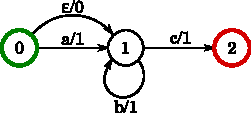
\includegraphics[width=72mm]{figures/WFSA}
  \end{center}
  \vfill
  Represents {\tt a?b*c} and the score of each string is its length.
\end{frame}

\begin{frame}{Weighted Finite-State Transducers}{}
  A \alert{weighted finite-state transducer} compactly represents a
  relation between two sets of strings, with a score assigned to each
  output string.
  \vfill
  Formally, a WFST comprises
  \begin{description}
  \item[states] some of which are start states, end states, or both;
    and
  \item[edges] between states, labeled with input symbols from a
    finite alphabet, output samples from a (potentially different)
    finite alphabet, and scores.
  \end{description}
\end{frame}

\begin{frame}{An Example}{}
  \begin{center}
    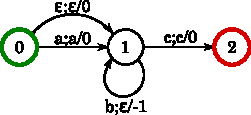
\includegraphics[width=72mm]{figures/WFST}
  \end{center}
  \vfill
  Maps strings in {\tt a?b*c} to {\tt a?c} by deleting {\tt b} symbols
  and the score of each string the change in its length.
\end{frame}

\begin{frame}{Composition}{}
  \begin{center}
    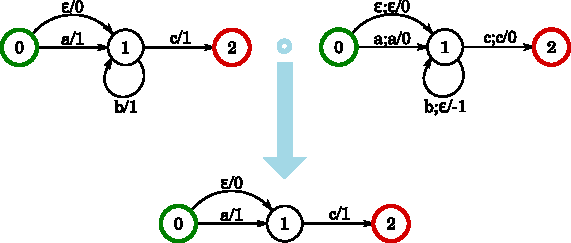
\includegraphics[width=96mm]{figures/Composition}
  \end{center}
  \vfill
  Given WFSA $\mathcal{S}$ and WFST $\mathcal{T}$, their composition
  $\mathcal{T} \circ \mathcal{S}$ is a WFSA that represents the set of
  strings (and corresponding scores) obtained by applying
  $\mathcal{T}$ to the set of strings represented by $\mathcal{S}$.
\end{frame}

\begin{frame}{Roadmap for WFST-based keyword search}{}
  \begin{enumerate}
  \item Form a WFST index representing a relation between
    \begin{description}
      \item[inputs] all high-probability strings of words or phones in
        the collection,
      \item[outputs] times of occurrence of the words or phones, and
      \item[scores] probabilities of the strings;
    \end{description}
    \item Form a WFSA representing a query; then
    \item \alert{compose} the query WFSA with the index WFST to
      perform the search.
  \end{enumerate}
\end{frame}

%% WFST search:  index generation (token and phonetic)
\begin{frame}{Building an index}{1. Generate a lattice for each segment in the collection.}
  \begin{center}
    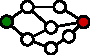
\includegraphics[width=36mm]{figures/lattice}
  \end{center}
  \begin{overlayarea}{\textwidth}{24mm}
    \begin{columns}[t]
      \column{54mm}
      \onslide<1>{
        \centerline{\bf Lattice}
        \begin{description}
        \item[Nodes] times
        \item[Edges] words (or phones) and posterior probabilities
        \end{description}
      }
      \column{54mm}
      \onslide<2>{
        \centerline{\bf Transducer}
        \begin{description}
        \item[Inputs] words (or phones)
        \item[Outputs] times
        \item[Scores] negative log-posteriors
        \end{description}
      }
    \end{columns}
  \end{overlayarea}
\end{frame}

\begin{frame}{Building an index}{2. Produce the factor automaton for each segment.}
  \begin{center}
    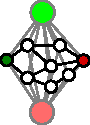
\includegraphics[width=36mm]{figures/factor}
    \end{center}
  \vfill
  Added edges have $\epsilon$ inputs, $\epsilon$ outputs, and no costs.
\end{frame}

\begin{frame}{Building an index}{3. Connect all the factor automata in parallel.}
  \begin{center}
    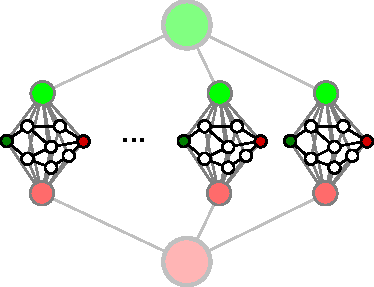
\includegraphics[width=66mm]{figures/index}
    \end{center}
  \vfill
  Added edges from start have $\epsilon$ inputs, segment ID outputs, and no costs.
  Added edges to end have $\epsilon$ inputs, $\epsilon$ outputs, and no costs.
\end{frame}

\begin{frame}{Building a query}{}
  In-vocabulary queries are simple:
  \begin{enumerate}
  \item use a word-based WFST index, and
  \item represent queries as word-level linear-chain WFSAs.
  \end{enumerate}
  \vfill
  Queries containing \alert{out-of-vocabulary} words are more challenging.
\end{frame}

\begin{frame}{Handling out-of-vocabulary queries}{}
  \begin{enumerate}
  \item represent queries as phone-level linear-chain WFSAs,
  \item compose the WFSAs with a WFST \alert{confusability} model,
  \item prune the resulting WFSAs, and
  \item {\bf if a word-based index is used}, compose the query WFSAs
    with a WFST that maps phone sequences back to words.
  \end{enumerate}
  \vfill
  The confusability model is created by running speech recognition on
  the training data and counting co-occurrences of reference and
  hypothesized phones.
  \vfill
  \nb{This is a form of query expansion, which is well
    studied in the information retrieval literature.}
\end{frame}

\begin{frame}{How do we measure keyword search performance?}
  {Actual Term-Weighted Value (ATWV)}
  \begin{equation*}
    \text{ATWV}(\theta) = \frac{1}{N}\sum_{q}
    \left[
      \frac{N_{\text{hit}}(q;\theta)}{N_{\text{true}}(q)} -
      \beta \frac{N_{\text{FA}}(q;\theta)}{T - N_{\text{true}}(q)}
      \right]
  \end{equation*}
  \begin{itemize}
  \item There are $N$ test queries indexed by $q$,
  \item $\theta$ is a decision threshold,
  \item $N_{\text{hit}}(q;\theta)$ is the number of correct detections and
  \item $N_{\text{FA}}(q;\theta)$ is the number of false alarms for
    query $q$ at decision threshold $\theta$, 
  \item $N_{\text{true}}(q)$ is the number of occurrences of query $q$
    in the test audio,
  \item $T$ is the duration of the test audio in seconds, and
  \item $\beta = 999.9$ is a weight on the penalty for false alarms.
  \end{itemize}
\end{frame}

\begin{frame}{Breaking it down}{}
  \begin{overlayarea}{\textwidth}{56mm}
  \only<1>{
  \begin{equation*}
    \text{ATWV}(\theta) = \frac{1}{N}\sum_{q}
    \left[
      {\color{red}\frac{N_{\text{hit}}(q;\theta)}{N_{\text{true}}(q)}} -
      \beta \frac{N_{\text{FA}}(q;\theta)}{T - N_{\text{true}}(q)}
      \right]
  \end{equation*}
  }
  \only<2>{
  \begin{equation*}
    \text{ATWV}(\theta) = \frac{1}{N}\sum_{q}
    \left[
      \frac{N_{\text{hit}}(q;\theta)}{N_{\text{true}}(q)} -
      {\color{red}\beta \frac{N_{\text{FA}}(q;\theta)}{T - N_{\text{true}}(q)}}
      \right]
  \end{equation*}
  }
  \only<3>{
  \begin{equation*}
    \text{ATWV}(\theta) = \frac{1}{N}\sum_{q}
    \left[
      \frac{N_{\text{hit}}(q;\theta)}{N_{\text{true}}(q)} -
      \beta \frac{N_{\text{FA}}(q;\theta)}{T - N_{\text{true}}(q)}
      \right]
  \end{equation*}
  }
  \vspace*{8mm}
  \begin{itemize}
  \item<1-> Hits earn a reward of $\frac{1}{N \cdot N_{\text{true}}(q)}$, so
    rare terms are more valuable.
  \item<2-> False alarms incur a constant loss of approximately
    $\frac{\beta}{N \cdot T}$ (because $T \gg N_{\text{true}}(q)$ for all $q$).
  \item<3-> Perfect performance scores $\text{ATWV} = 1.0$, while
    empty output scores $\text{ATWV} = 0.0$.  $\text{ATWV} < 0.0$
    means you have too many false alarms!
  \end{itemize}
  \end{overlayarea}
  \vfill
  \nb{Score normalization is important under the ATWV metric.  For
    more details on this issue, please see \cite{Wang2014}.}
\end{frame}

\begin{frame}{Babel Languages}{}
  \begin{center}
    \begin{tabular}{@{}llll@{}} \toprule
      \multicolumn{1}{c}{\bf Period 1} & \multicolumn{1}{c}{\bf Period 2} & \multicolumn{1}{c}{\bf Period 3} & \multicolumn{1}{c}{\bf Period 4} \\ \midrule
      Cantonese  & Assamese       & Kurmanji Kurdish & Pashto \\
      Pashto     & Bengali        & Tok Pisin        & Guaran\'{i} \\
      Turkish    & Haitian Creole & Cebuano          & Igbo \\
      Tagalog    & Lao            & Kazakh           & Amharic \\
      Vietnamese & Zulu           & Telugu           & Mongolian \\
                 & Tamil          & Lithuanian       & Javanese \\
                 &                & Swahili          & Dholuo \\
                 &                &                  & Georgian \\ \bottomrule
    \end{tabular}
  \end{center}
\end{frame}

\begin{frame}{What language characteristics matter?}{}
  \begin{enumerate}
  \item Morphology
  \item Writing system
  \item Tonal languages
  \end{enumerate}
\end{frame}

%% Morphology and vocabulary growth
\begin{frame}{Morphology}{}
  The morphology of a language refers to the structure of its words.
  Specifically, are words atomic, or are they composed from meaningful
  parts?
  \vfill
  {\color{DarkerBlue}\bf English example} \\
  re+ +do+ +er --- one who is performing some action again
  \vfill
  Languages with \alert{agglutinative} morphology have large
  inventories of words formed by the composition of smaller units
  (morphs).
  \vfill
  One way to characterize this is through vocabulary growth.
\end{frame}

\begin{frame}{Vocabulary Growth for Babel Languages}{}
  \begin{center}
    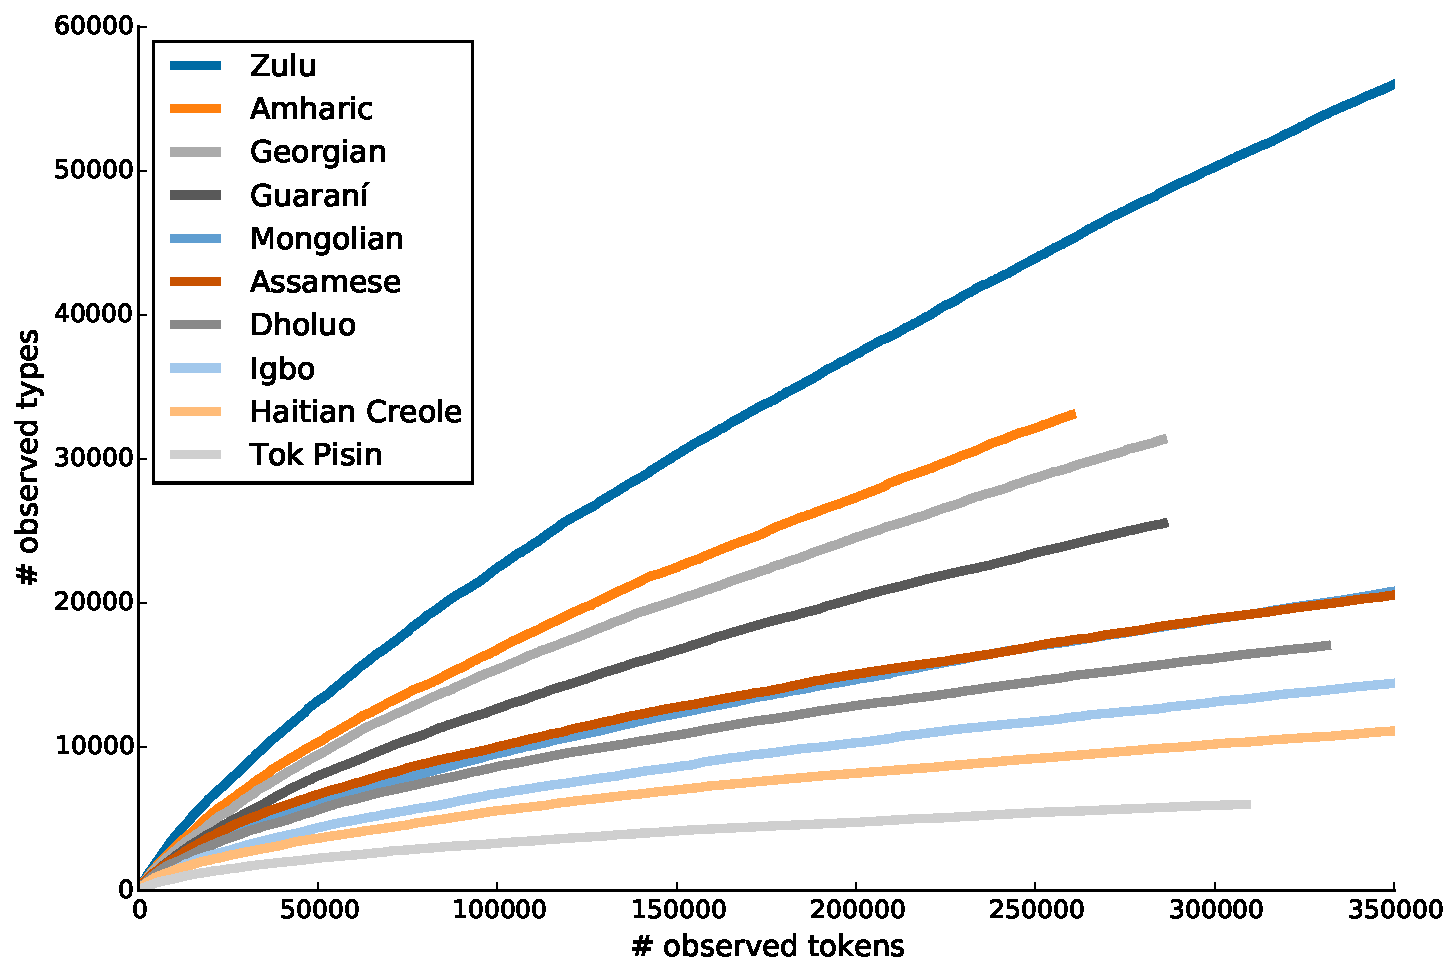
\includegraphics[width=108mm]{figures/vocGrowth}
  \end{center}
\end{frame}

\begin{frame}{Mitigating Rapid Vocabulary Growth}{}
  Out-of-vocabulary words are more likely to occur in test data for
  languages with rapid vocabulary growth, which will degrade speech
  recognition and keyword search performance.
  \vfill
  Two ways to reduce the impact:
  \begin{description}[morph models]
    \item[morph models] base the vocabulary on morphs instead of
      words, and
    \item[web text] expand the vocabulary by collecting text from the
      web.
  \end{description}
\end{frame}

\begin{frame}{Morph Models}{}
  Recipe:
  \begin{enumerate}
  \item Segment the training text into morph-like units using
    Morfessor~\cite{Morfessor} or some other tool.
  \item Generate a pronunciation lexicon for the morphs.
  \item Train a language model on the segmented training text.
  \end{enumerate}
  \vfill
  Task-specific considerations:
  \begin{description}
  \item[ASR]
    \begin{itemize}
    \item Recomposing morphs into words is challenging.
    \end{itemize}
  \item[KWS]
    \begin{itemize}
      \item Need to decompose queries into morphs.
      \item Best results obtained by doing word and morph search, and
        fusing the results.
    \end{itemize}
  \end{description}
\end{frame}

\begin{frame}{Keyword Search Results with Morph Models}{}
  \begin{columns}[c]
    \column{68mm}
    \centering
    \begin{tabular}{@{}lcc@{}} \toprule
      & {\bf Word} & {\bf Word+Morph} \\
      {\bf Language} & {\bf MTWV} & {\bf MTWV} \\ \midrule
      Zulu     & 0.1817 & 0.2305 \\
      Assamese & 0.2643 & 0.2797 \\ \bottomrule
    \end{tabular}
    \column{40mm}
    \centering{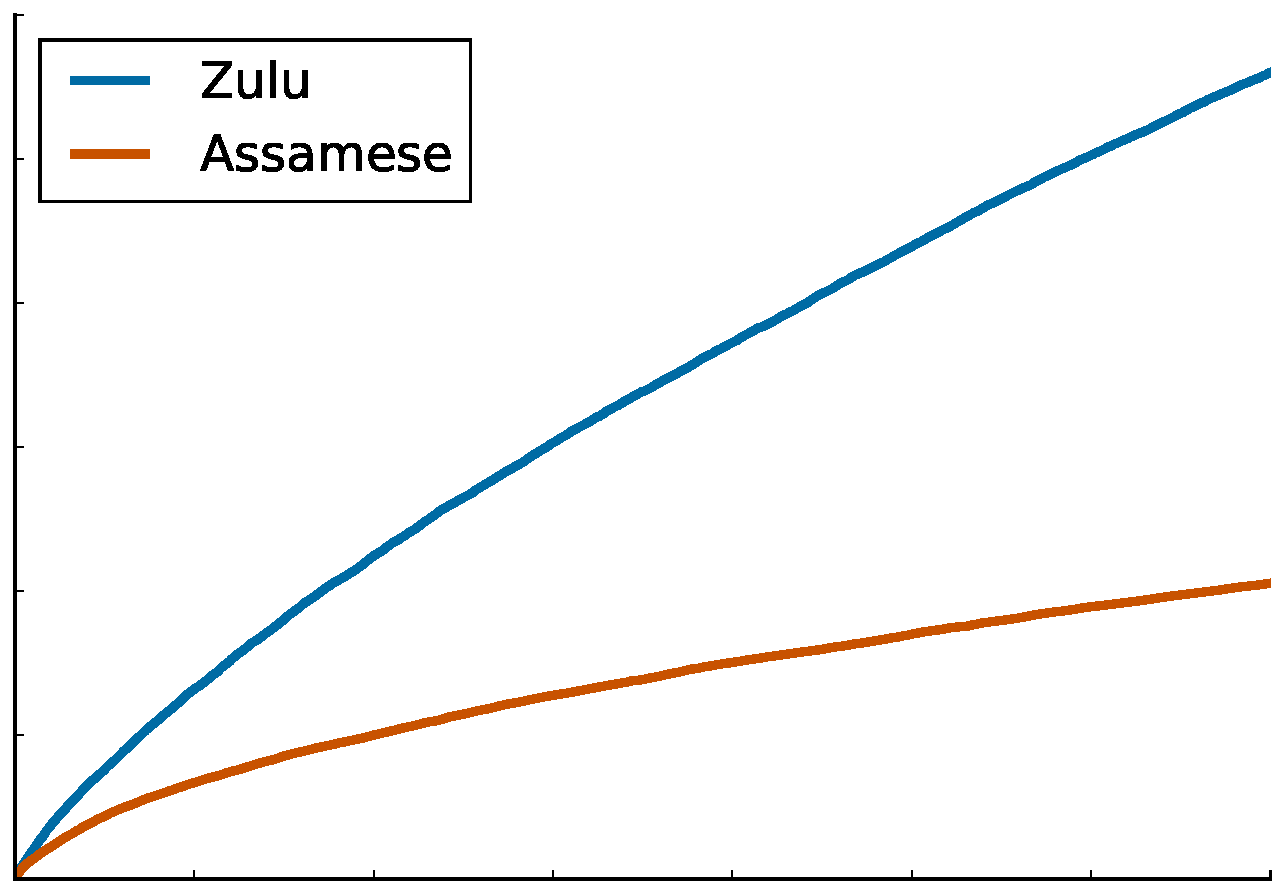
\includegraphics[width=40mm]{figures/vocGrowthThumb}}
  \end{columns}
  \vfill
  \nb{Maximum Term-Weighted Value (MTWV) is ATWV with an oracle
    decision threshold.}
\end{frame}

\begin{frame}{Web Text}{}
  General considerations:
  \begin{itemize}
  \item How much web presence does the language have?
    \begin{itemize}
    \item Swahili: plenty
    \item Dholuo: sparse
    \end{itemize}
  \item How easy is it to generate queries returning the target language?
    \begin{itemize}
    \item Amharic has its own Unicode range, so it is easy.
    \item Tagalog contains many English and Spanish loanwords, so it
      is difficult.
    \end{itemize}
  \item Normalization is a must!
  \end{itemize}
\end{frame}

\begin{frame}{Web Text}{}
  Task-specific considerations:
  \begin{description}
  \item[ASR] Improvements may be small due to genre mismatch (LM is important).
  \item[KWS] Better vocabulary coverage improves performance (LM is not important).
  \end{description}
\end{frame}

\begin{frame}{Impact of Web Text}{}
  \centering
  \begin{tabular}{@{}lcd{6.1}d{3.1}cc@{}} \toprule
    & & \multicolumn{1}{c}{\bf Train} & \multicolumn{1}{c}{\bf Voc.} &               &            \\
    {\bf Language} & {\bf Web?} & \multicolumn{1}{c}{\bf size} & \multicolumn{1}{c}{\bf size} & {\bf \% WER} & {\bf MTWV} \\ \midrule


    Igbo        & N &     45.3 & 16.5 & 66.5 & 0.2387 \\
                & Y &  17200.  & 19.5 & 66.5 & 0.2389 \\ \midrule
    Guaran\'{i} & N &     46.8 & 26.3 & 53.5 & 0.4562 \\
                & Y &  23900.  & 36.9 & 53.5 & 0.4665 \\ \midrule
    Mongolian   & N &     51.2 & 23.6 & 61.1 & 0.3497 \\
                & Y & 118000. & 220. & 60.4 & 0.3849 \\ \bottomrule
  \end{tabular}
  \vfill
  \raggedright
  Word counts are in thousands.
\end{frame}

\begin{frame}{How the Writing System Affects Lexicon Design}{}
  We will discuss four types of writing system:
  \begin{description}[logographic]
  \item[logographic] Large character inventory, with each
    character representing a morpheme, e.g. Chinese.
  \item[alphabetic] Small character inventory, with characters
    representing phonemes, e.g. Javanese.
  \item[abjad] Small character inventory, with characters representing
    consonants and long vowels, e.g. Pashto.
  \item[abugida] Medium character inventory, with characters
    representing consonant-vowel sequences, e.g. Amharic.
  \end{description}
\end{frame}

\begin{frame}{Lexicons for Logographic Writing Systems}{}
  Unless you have thousands of hours of transcribed data, you must
  have a phonetic dictionary of characters.
\end{frame}

\begin{frame}{Lexicons for Alphabets}{}
  {\color{DarkerBlue}\bf Graphemic approach} \\
  The pronunciation of a word is its letter sequence.  Use if
  \begin{itemize}
  \item you have no other information about the relationship between
    spelling and sound, or
  \item the writing system is phonetic, as in Turkish or Georgian.
  \end{itemize}
  \vfill
  {\color{DarkerBlue}\bf Approximate phonetic approach} \\
  Use WFST to convert letter sequences to sound sequences.      
\end{frame}

\begin{frame}{Javanese Spelling-to-sound}{}
  Javanese uses the Latin alphabet.  Most letters have a single
  pronunciation (phonetic writing), but there are digraphs that
  correspond to single phonemes:
  \vfill
  \centering
  \begin{tabular}{@{}l@{$\rightarrow$}l@{}}
    th & t` \\
    dh & d` \\
    ny & J  \\
    ng & N  \\
    sy & S  \\
  \end{tabular}
  \vfill
  \raggedright
  Use a greedy, WFST-based pronunciation generator.
\end{frame}

\begin{frame}{Javanese Spelling-to-sound}{}
  \centering
  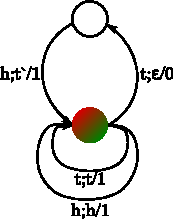
\includegraphics[width=36mm]{figures/Javanese}
  \vfill
  \raggedright
  Compose each word with transducer and pick the output with the
  lowest score (length).
  \vfill
  \nb{The diagram is a sketch that omits many transitions.}
\end{frame}

\begin{frame}{Lexicons for Abjads}{}
Use the same approach as for alphabets, but what about the unwritten
vowels?
\vfill
\begin{description}[Ignore them]
\item[Ignore them] Simple, and usually works fine.
\item[Infer them] Feasible only with lots of transcribed data.
\end{description}
\end{frame}

\begin{frame}{Lexicons for Abugidas}{}
In general, each character will map to a consonant-vowel pair.  The
details will be language-dependent. \\
In Amharic each Unicode code point denotes a syllable:
\vfill
\centering
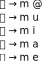
\includegraphics[height=24mm]{figures/Amharic}
\vfill
\raggedright
In such cases, a lookup table is enough.
\end{frame}

\begin{frame}{Lexicons for Abugidas}{}
In many Indian languages, such as Telugu, characters have a
default vowel that can be modified by the following character.
\vfill
\centering
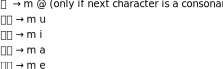
\includegraphics[height=24mm]{figures/Telugu}
\vfill
\raggedright
In these cases, a WFST framework is the best approach.
\vfill
\nb{In the list above, the first Telugu glyph is generated by one
  Unicode code point, but the others are generated by two.}
\end{frame}

\begin{frame}{Tonal Languages}{}
  \alert{Tonal} languages use pitch (and phonation in some cases)
  to convey lexical or grammatical information.  Tone information
  might or might not be indicated in the writing system:
  \vfill
  \begin{description}[Not written]
  \item[Written] Cantonese, Vietnamese, Lao
  \item[Not written] Zulu, Igbo, Dholuo
  \end{description}
\end{frame}

\begin{frame}{Tonal Languages}{}
  If tone is indicated in the writing system, the front end needs to
  represent pitch either
  \begin{itemize}
  \item explicitly (e.g., using FFV features~\cite{Laskowski2008}), or
  \item implicitly (e.g., using high-resolution Mel spectra).
  \end{itemize}
  \vfill
  \centering
  \begin{tabular}{@{}lc@{}} \toprule
    {\bf Features} & {\bf \% WER} \\ \midrule
    PLP & 63.3 \\
    +FFV & 60.6 \\ \bottomrule
  \end{tabular}
  \vfill
  \raggedright
  Results on Lao, using a 10-hour training set.
\end{frame}

% Recipe for a new language, illustrated with Guarani
\begin{frame}{A Recipe for a New Language: Paraguayan Guaran\'{i}}{}
  \begin{itemize}
    \item Background on the language
    \item Dictionary generation
    \item Training acoustic models
    \item Training language models
    \item Performance comparisons
  \end{itemize}
\end{frame}

% Background
\begin{frame}{Paraguayan Guaran\'{i}}{}
  \begin{columns}[c]
    \column{46mm}
    \begin{itemize}
    \item An official language in Paraguay
    \item Tupian language family
    \item Around 4 million native speakers
    \item Substantial Spanish influence: code-switching and calques
    \end{itemize}
    \column{62mm}
    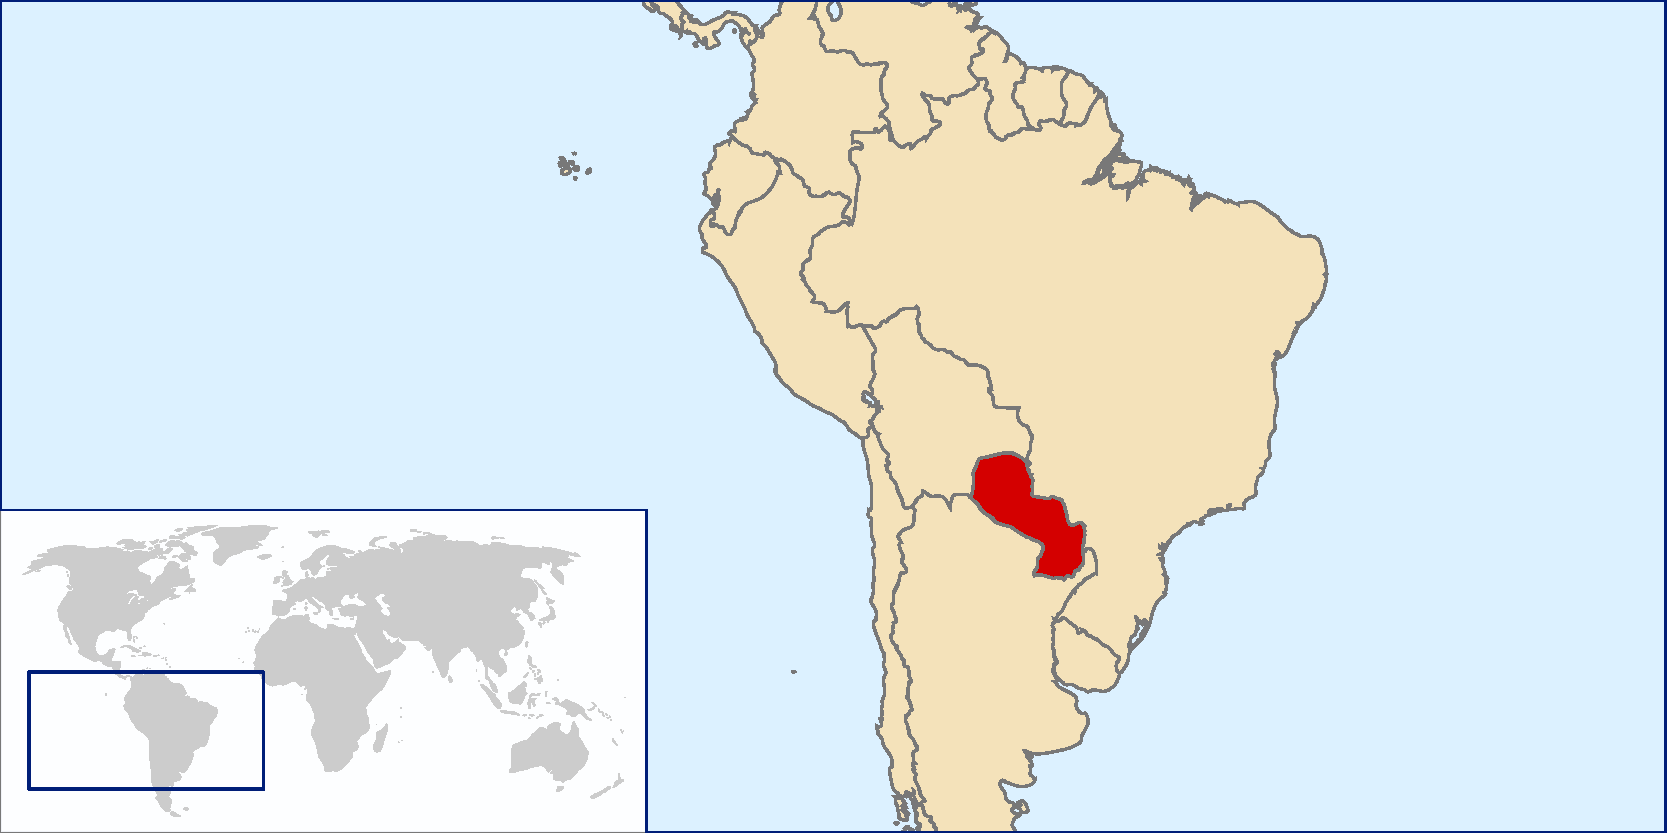
\includegraphics[width=62mm]{figures/LocationParaguay}
  \end{columns}
  \vfill
  \nb{Map of Paraguay by Wikimedia user \href{https://commons.wikimedia.org/wiki/User:Rei-artur}{Rei-artur}}
\end{frame}

\begin{frame}{Dictionary Generation}{The Guaran\'{i} writing system}
  \begin{itemize}
  \item Latin alphabet
  \item `w' only in loan words
  \item apostrophe marks glottal stops
  \item Tilde can appear on eight letters
    \begin{itemize}
    \item \~{a}, \~{e}, \~{\i}, \~{o}, \~{u}, \~{y}, \~{g}, and \~{n}
    \end{itemize}
  \item Acute accent can appear on six letters
    \begin{itemize}
    \item \'{a}, \'{e}, \'{\i}, \'{o}, \'{u}, \'{y}
    \end{itemize}
  \item Dieresis can appear on `u'
    \begin{itemize}
    \item \"{u}
    \end{itemize}
  \item Ten digraphs
    \begin{itemize}
    \item mb, nd, ng, and nt (prenasalized consonants)
    \item \~{g} (Unicode Latin Small Letter G and Unicode Combining Tilde)
    \item ch, sh, and qu
    \item rr and ll (only in Spanish loan words)
    \end{itemize}
  \end{itemize}
\end{frame}

\begin{frame}{Sample Lexicon Entries}{Regular words}
  \centering
  \begin{tabular}{@{}ll@{}}
    emba'apomi\'{e}ma(01) & e mb a ' a p o m i e' m a \\
    hasyp\'{a}ma(01) & h a s y p a' m a \\
    mb\'{o}i(01) & mb o' i \\
    nopenamo'\~{a}i(01) & n o p e n a m o ' a\~{} i \\
    ofalla'imi(01) & o f a ll a ' i m i \\
    o\~{n}ak\~{a}kar\~{a}i(01) & o n\~{} a k a\~{} k a r a\~{} i \\
    pack(01) & p a k \\
    rohechaga'ueterei(01) & r o h e ch a g a ' u e t e r e i \\
    veintinu\'{e}ve(01) & v e i nt i n u e' v e \\
    \~{n}a\~{n}omongeta(01) & n\~{} a n\~{} o m o ng e t a \\
  \end{tabular}
\end{frame}

\begin{frame}{Pronunciations of Spellings}{}
  The data includes spellings, which are marked with underscores, e.g. ``a\_m.''
  \vfill
  In Guaran\'{i}, spellings are usually given with
  Spanish letter pronunciations, except for nasalized vowels and
  \~{g}.
  \vfill
  We opted to generate both Spanish and Guaran\'{i} pronunciations for
  spelled tokens.
\end{frame}

\begin{frame}{Sample Lexicon Entries}{Spellings}
  \centering
  \begin{tabular}{@{}ll@{}}
    a\_m(01)    & ' a' ' e' m e\~{} \\
    a\_m(02)    & ' a' m e\~{} \\
    b\_c(01)    & b e' s e' \\
    b\_r(01)    & b e' ' e' r e \\
    b\_r(02)    & b e' r e' \\
    c\_n\_c(01) & s e' ' e' n e\~{} s e' \\
    c\_n\_c(02) & s e' n e\~{} s e' \\
    e\_p\_p(01) & ' e' p e' p e' \\
    j\_r\_h(01) & h o' t a ' e' r e ' a' ch e \\
    j\_r\_h(02) & j e' r e' h e' \\
  \end{tabular}
\end{frame}

\begin{frame}{Training Acoustic Models}{}
  \begin{itemize}
  \item Flat start: bootstrapping the models
  \item Monolingual deep neural network model
  \item Multilingual deep neural network model
  \end{itemize}
\end{frame}

% flat start
\begin{frame}{Flat Start}{}
  \centering
  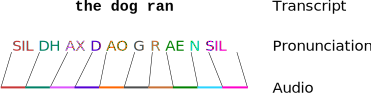
\includegraphics[width=96mm]{figures/FlatStart}
  \vfill
  \raggedright
  \begin{overlayarea}{\textwidth}{48mm}
    \begin{enumerate}
    \item Initialize single-Gaussian models with uniform segmentation
    \item Run many iterations of forward-backward training
    \item Gradually increase the number of mixture components
    \end{enumerate}
    \only<2>{
      Two pitfalls:
      \begin{itemize}
      \item Need for a garbage (REJ) model
      \item Inclusion of long silences within segments
      \end{itemize}
    }
  \end{overlayarea}
\end{frame}

\begin{frame}{Our Recipe}{}
  \begin{description}[Context-Independent]
  \item[GMM] 80 passes over data, splitting mixtures every 8.
  \item[Speech/Nonspeech] 
    \begin{enumerate}
    \item Seed SPEECH, SIL, and REJ models with GMM.
    \item 5 iterations Viterbi training, skipping utterances
      containing REJ.
    \end{enumerate}
  \item[Context-Independent]
    \begin{enumerate}
    \item Seed phone models with SPEECH.
    \item 5 iterations forward-backward training, skipping utterances
      containing REJ.
    \end{enumerate}
  \end{description}
  \vfill
  These models use PLP$+\Delta+\Delta^{2}$ features.
\end{frame}

\begin{frame}{Our Recipe}{}
  \begin{description}[Phonetic mixup] 
  \item[Phonetic mixup] Train 3 successive models
    \begin{enumerate}
    \item 250 states; 6 mixtures per state
    \item 500 states; 6 mixtures per state
    \item 1,000 states; 6 mixtures per state
    \end{enumerate}
    Training is 20 iterations of Viterbi, then 10 iterations of
    forward-backward.
  \item[Global mixup] Train 3 successive models, each with 1,000
    states and 6 mixtures per state.
  \item[Full model] 6,000 states and 6 mixtures per state
  \end{description}
  \vfill
  These models use PLP+LDA+STC features. \\
  Phonetic models use phone+position roots for decision trees, while
  global and full models use position roots.
\end{frame}

% Monolingual DNN
\begin{frame}{Our Recipe}{Monolingual DNN}
  \begin{itemize}
  \item Input is 9 frames of 40-d PLP+LDA+STC features.
  \item 3 hidden layers with 1,024 ReLU units, then
  \item 1 hidden layer with 1,024 sigmoid units, then
  \item 128-unit linear bottleneck~\cite{Sainath2013}, then
  \item 3,000-unit softmax output layer.
  \end{itemize}
  \vfill
  Training on 40h of data in three phases:
  \begin{enumerate}
  \item discriminative pretraining~\cite{Seide2011},
  \item cross-entropy training, and
  \item state-level minimum Bayes risk training with distributed
    Hessian-free algorithm~\cite{Kingsbury2012}.
  \end{enumerate}
\end{frame}

% Multilingual DNN
\begin{frame}{Our Recipe}{Multilingual Features}
  \centering
  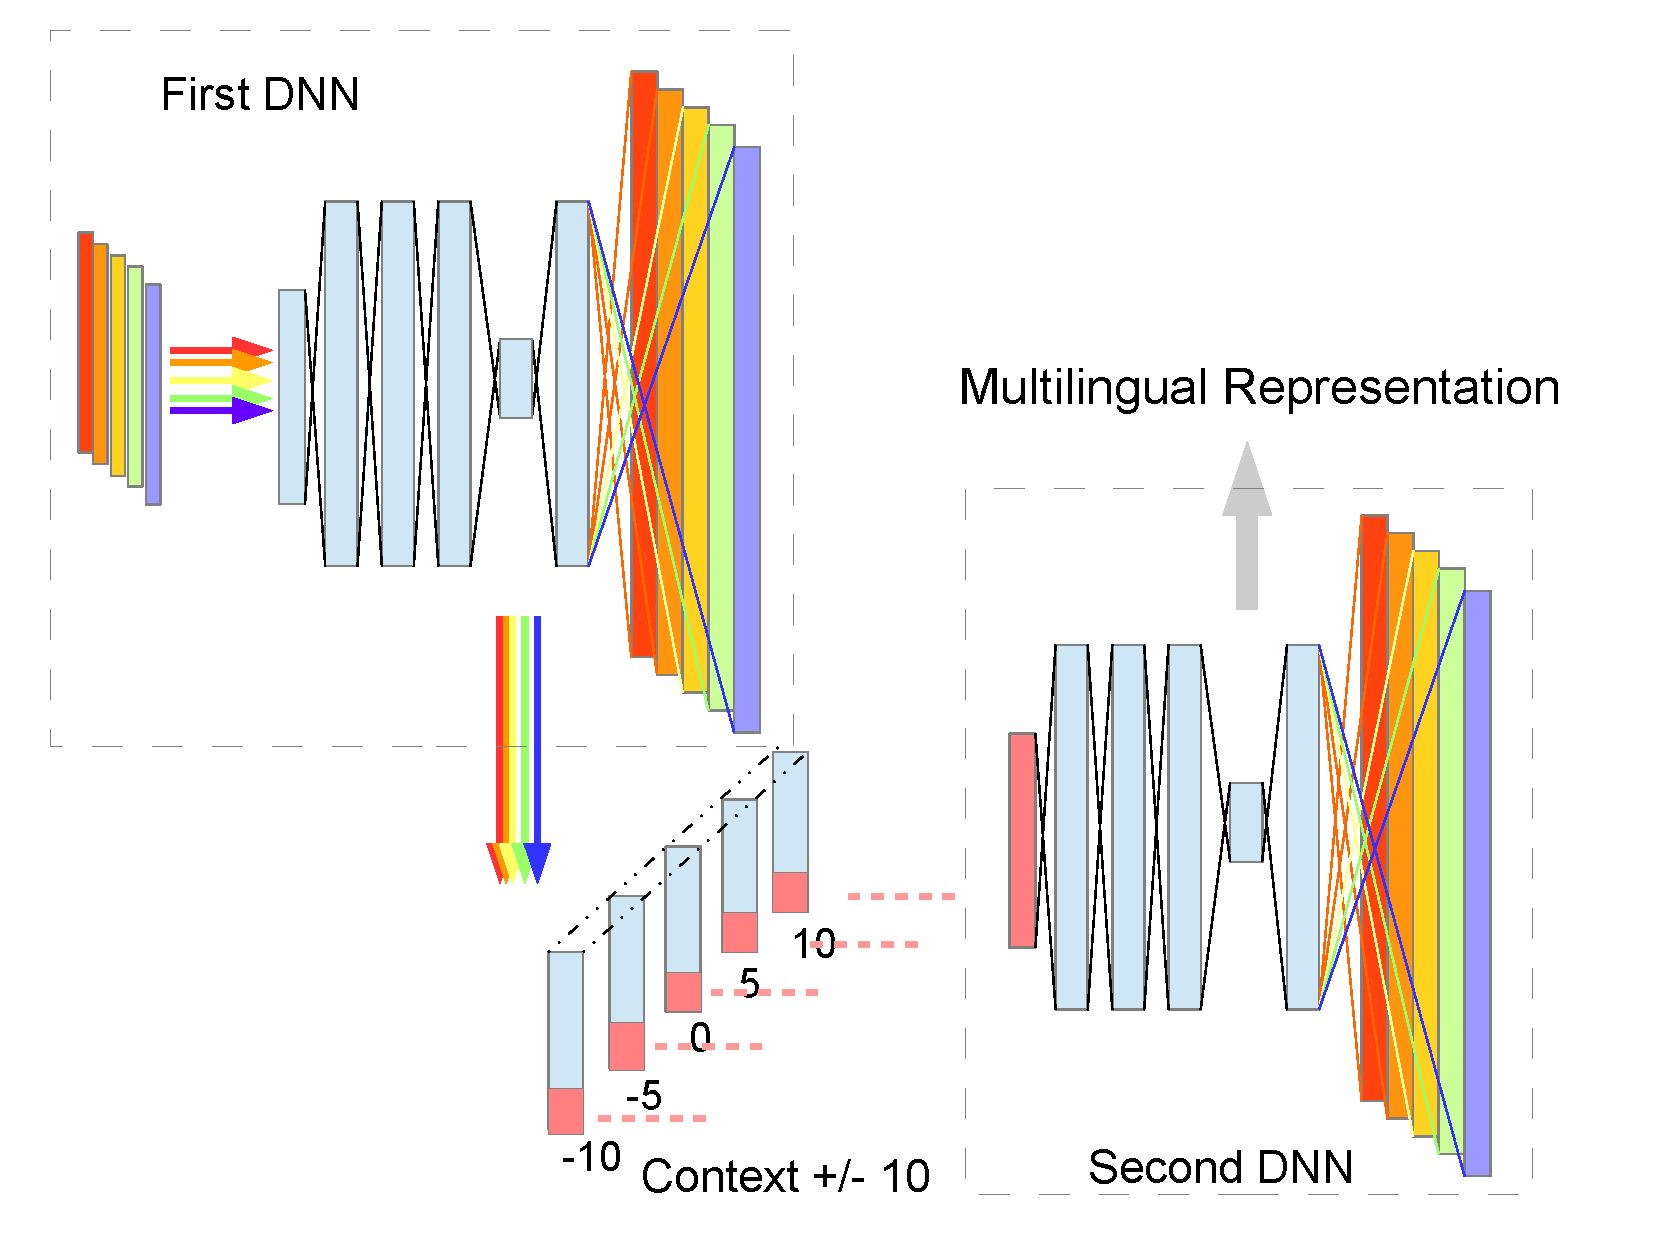
\includegraphics[height=48mm]{figures/mldnn}
  \vfill
  \raggedright
  Stacked CNN/DNN architecture similar to \cite{Grezl2009}, using
  language-dependent output layers~\cite{Scanzio2008}.
  \vfill
  \nb{Thanks to Jia Cui of IBM for this figure.}
\end{frame}

\begin{frame}{Our Recipe}{Multilingual Features}
  \begin{description}[CNN]
    \item[CNN]
      \begin{itemize}
      \item 11 frames of log-Mel$+\Delta+\Delta^{2}$ features
      \item Conv. layer with $9 \time 9$ kernels, 128 feature maps,
        and max-pooling in frequency with a window and stride of 3.
      \item Conv. layer with $3 \time 4$ kernels, 256 feature maps,
        and no pooling.
      \item 7 hidden layers of 2048, 1024, 1024, 1024, \alert{80},
        1024, and 3000 sigmoidal units.
      \end{itemize}
    \item[DNN]
      \begin{itemize}
      \item 80-d bottleneck output from CNN at $t-10$, $t-5$, $t$,
        $t+5$, and $t+10$.
      \item 5 hidden layers of 1024, 1024, \alert{80}, 1024, and 3000
        sigmoidal units.
      \end{itemize}
  \end{description}
  \vfill
  Training of all networks is cross-entropy on 24 Babel languages (all
  but Georgian).
\end{frame}

\begin{frame}{Our Recipe}{Multilingual DNN}
  \begin{itemize}
  \item Input is 1 frame of 80-d multilingual features.
  \item 3 hidden layers with 1,024 ReLU units, then
  \item 1 hidden layer with 1,024 sigmoid units, then
  \item 256-unit linear bottleneck, then
  \item 3,000-unit softmax output layer.
  \end{itemize}
  \vfill
  Training on 40h of data in three phases:
  \begin{enumerate}
  \item discriminative pretraining,
  \item cross-entropy training, and
  \item state-level minimum Bayes risk training with distributed
    Hessian-free algorithm.
  \end{enumerate}
\end{frame}

% LMs
\begin{frame}{Training Language Models}{}
  \begin{description}[On transcripts]
  \item[On transcripts] Bigram LM with modified Kneser-Ney smoothing
    trained on 320K words with a 26.3K vocabulary.
  \item[Plus web text] Interpolated bigram LM with modified Kneser-Ney
    smoothing trained on 17.2M words with a 36.9K vocabulary.
  \end{description}
\end{frame}

% Performance comparisons
\begin{frame}{Performance of different acoustic models}{}
  \centering
  \begin{tabular}{@{}lcc@{}} \toprule
  {\bf Model} & {\bf Multilingual?} & {\bf \% WER} \\ \midrule
  GMM      & N & 68.9 \\
  CE DNN   & N & 63.7 \\
  sMBR DNN & N & 58.3 \\
  sMBR DNN & Y &      \\ \bottomrule
  \end{tabular}
  \vfill
  \raggedright
  All runs use bigram LM trained from transcripts.
\end{frame}

\begin{frame}{Performance of different language models}{}
  \centering
  \begin{tabular}{@{}lcc@{}} \toprule
  {\bf Model} & {\bf \% WER} & {\bf MTWV} \\ \midrule
  Transcripts & & \\
  + Web text  & 47.5 & 0.5345 \\ \bottomrule
  \end{tabular}
  \vfill
  \raggedright
  All runs use multilingual DNN acoustic model.
\end{frame}


\section{New Domains}
\begin{frame}
  \begin{center}
    {\color{Maroon}\Huge Tackling a New Domain}
  \end{center}
\end{frame}

%% put section outline here


\section{Research Topics, Challenges, and New Ideas}

\begin{frame}
  \begin{center}
    {\color{Maroon}\Huge Research Directions and New Modeling Techniques}
  \end{center}
\end{frame}

%%%% ----------------------------
%%%%     CHALLENGES
%%%% ----------------------------

\begin{frame}
  \begin{center}
    {\color{Maroon}\Huge Challenges}
  \end{center}
\end{frame}

\begin{frame}{Are we there yet?}
  \begin{center}
    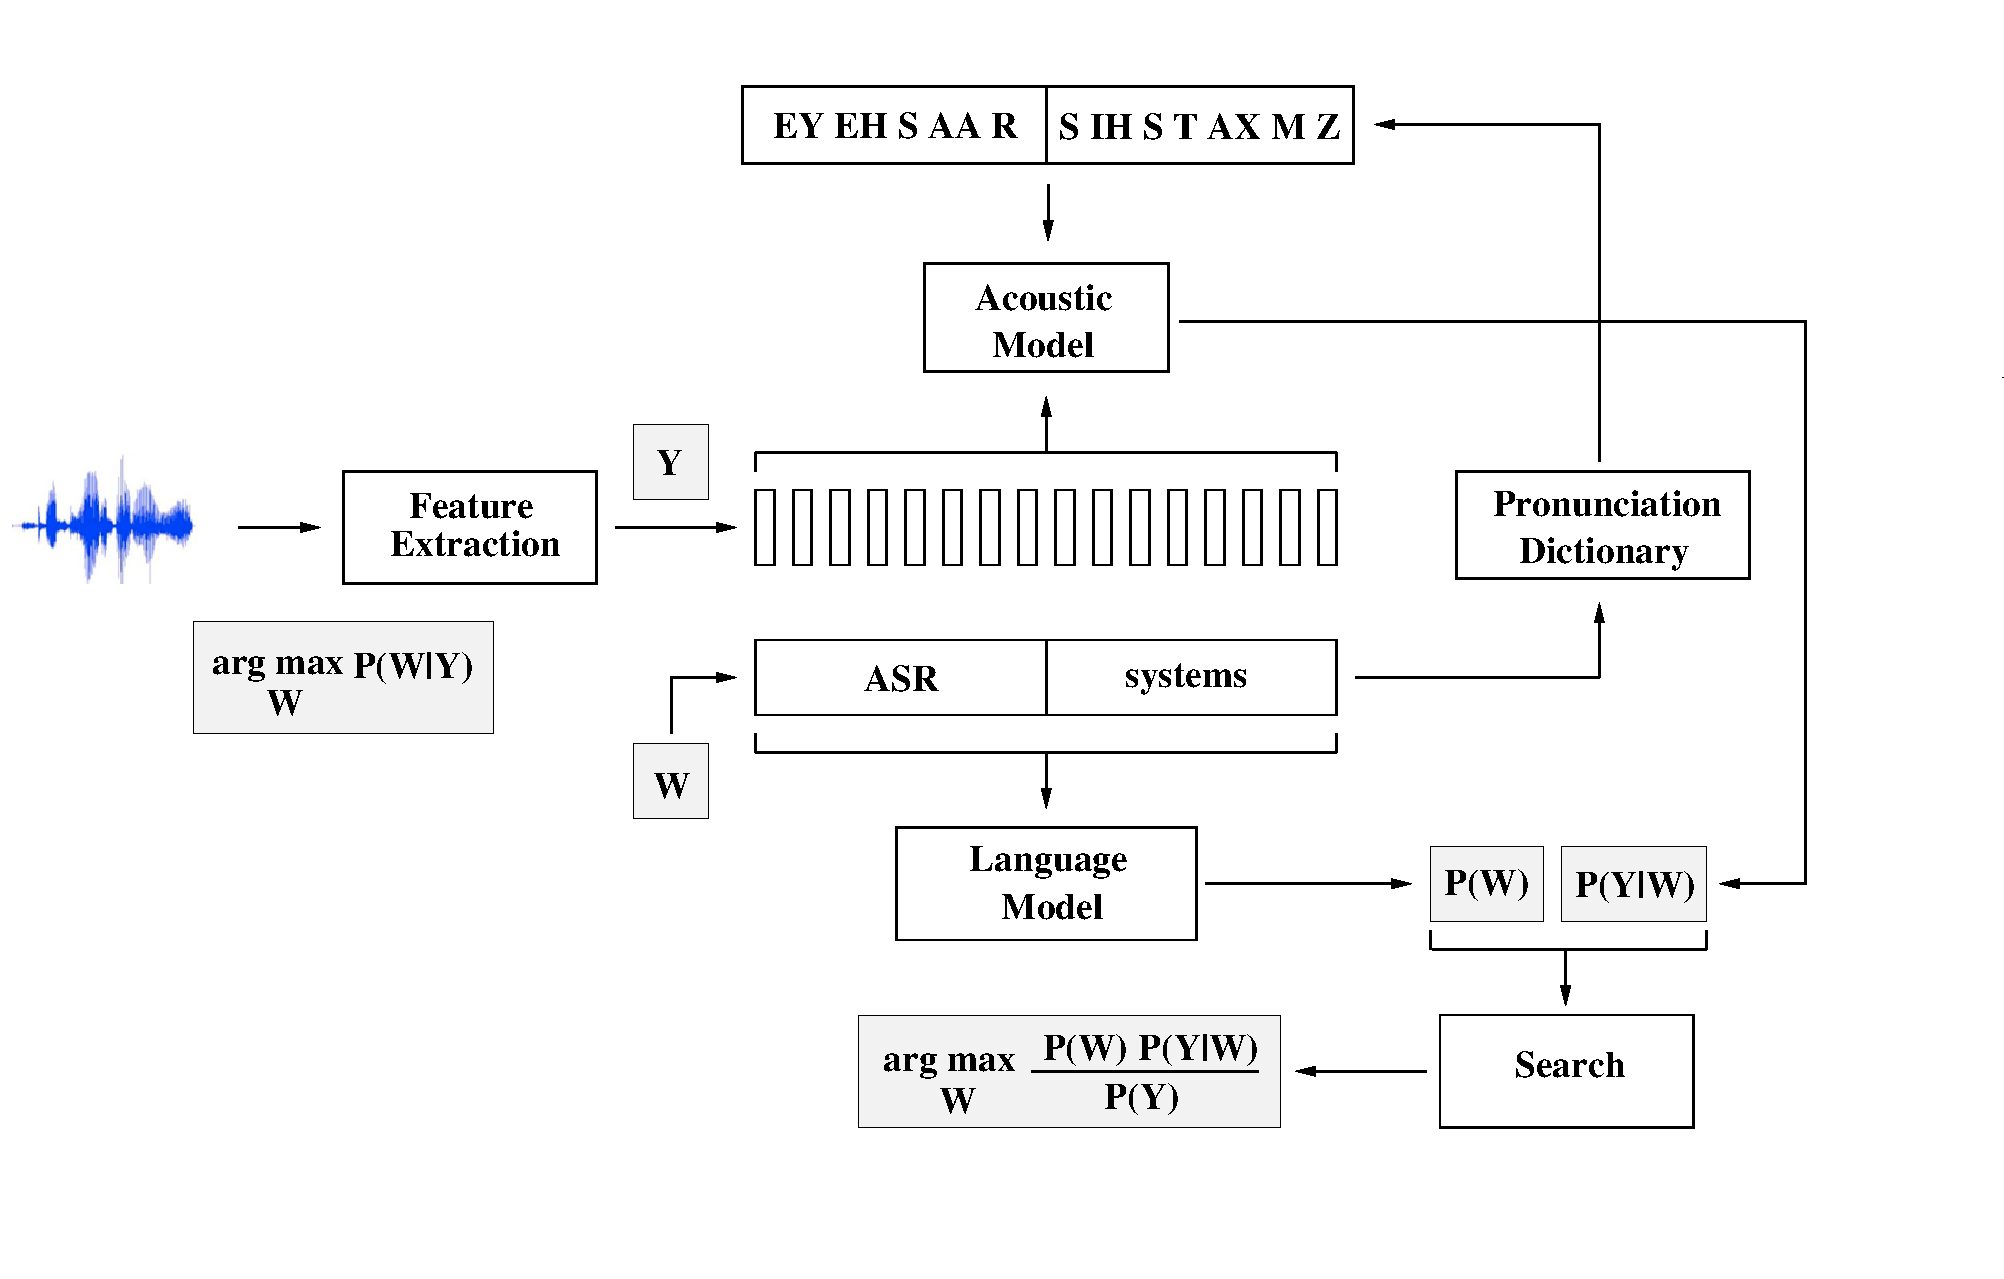
\includegraphics[height=77mm]{figures/ASR9}
  \end{center}
\end{frame}

\begin{frame}{Is that it?}
  \begin{center}
    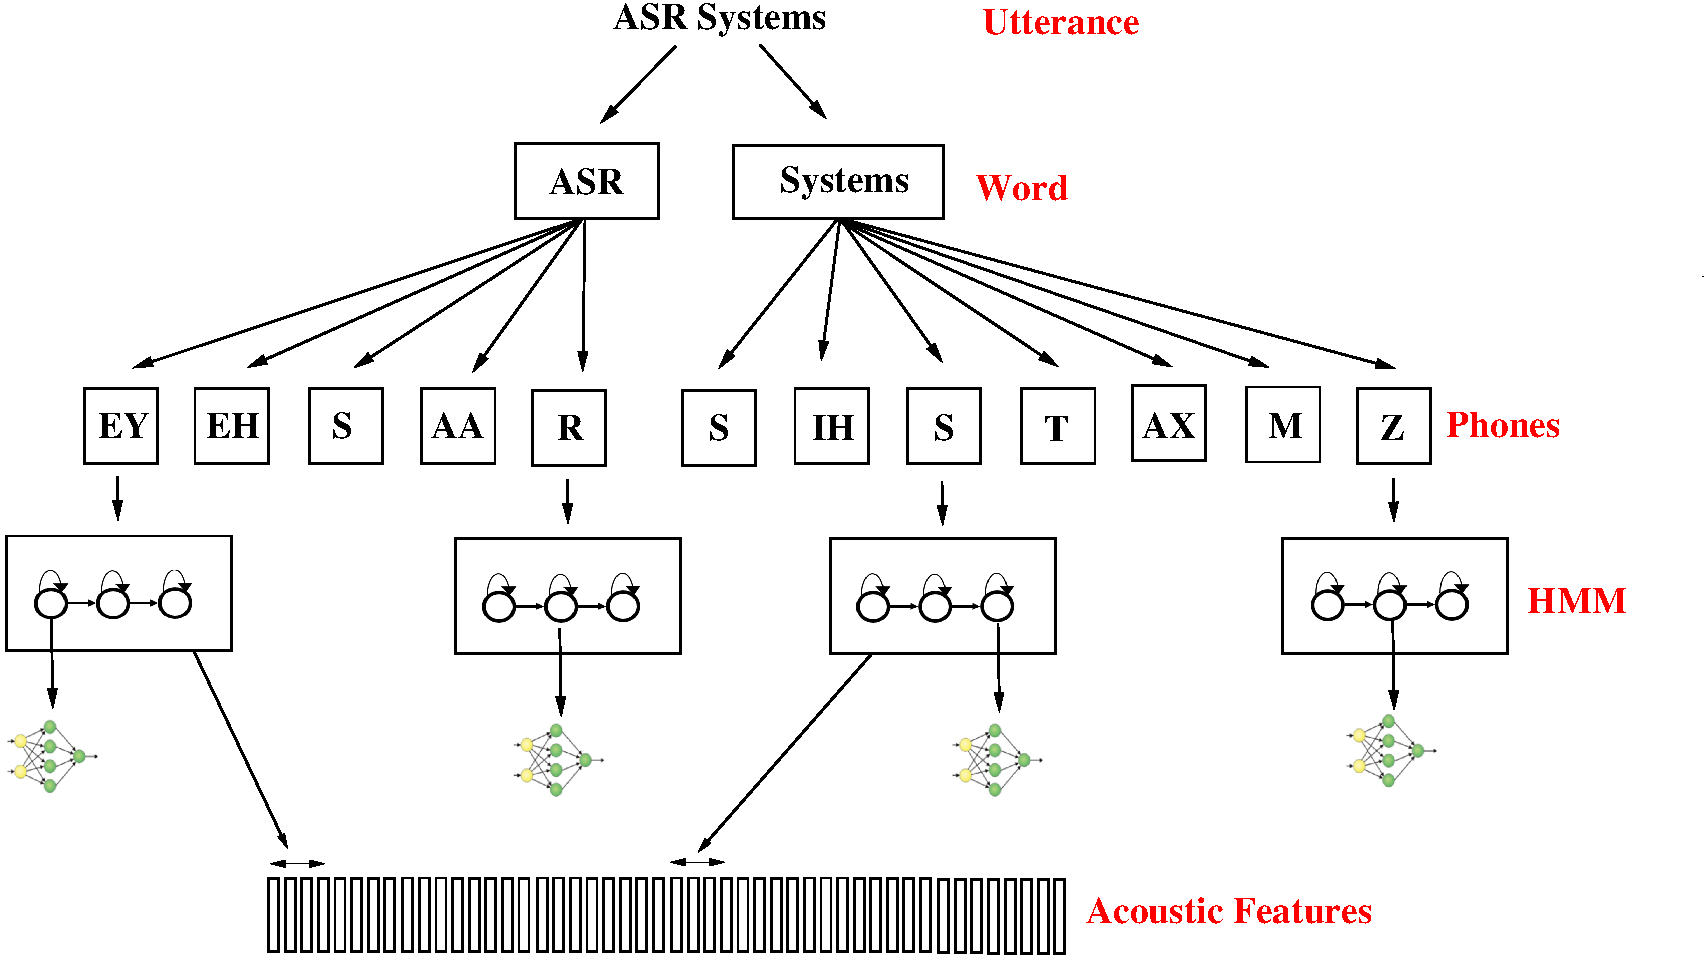
\includegraphics[height=65mm]{figures/am-mlp}
  \end{center}
\end{frame}

\begin{frame}{Challenges}
  \begin{itemize}
  \item What could be wrong?
  \item We are using a solid statistical framework, right?
  \item We know how to extract ``features''
  \item We know how to learn models
  \item We know how to search for the best path
  \end{itemize}
\end{frame}

\begin{frame}{Really?}
  \begin{itemize}
  \item Fundamental Equation of ASR
  \item $W' = argmax$
  \end{itemize}
\end{frame}

\begin{frame}
  \frametitle{Research Topics}
\end{frame}

\begin{frame}
  \frametitle{New Ideas}
\end{frame}

\section{End-to-End Systems}

\begin{frame}
  \frametitle{End-to-End Systems}
\end{frame}

\begin{frame}
  \begin{center}
    {\color{Maroon}\Huge Hands-On Experience with Virtual Machines}
  \end{center}
\end{frame}

\begin{frame}
  \frametitle{Practicalities}
  \begin{itemize}
  \item We want to give you hands-on experience with building ASR systems
  \item You will be able to train a system on a Babel language (most likely 201 Haitian)
  \item You can then experiment with other Babel languages, or port the system to other domains
  \item To facilitate experimentation, we will distribute a Virtual Machine (VM)
  \item \color{Maroon}Read on to see how you can prepare
  \end{itemize}
\end{frame}

\begin{frame}
  \frametitle{Virtual Machines and Tools}
  \begin{itemize}
  \item Think of a VM as a ``virtual'' computer, in our case running Linux
  \item VMs allow sharing reproducible experiments easily
  \item \url{https://github.com/srvk}, \url{http://speechkitchen.org} as repositories
  \item \url{https://www.vagrantup.com/} to build VMs
  \item \url{https://www.virtualbox.org/} to run VMs (along with \url{https://aws.amazon.com/})
  \item An ``image'' is a computer when it is turned off, it becomes an ``instance'' when you turn it on
  \end{itemize}
\end{frame}

\begin{frame}
  \frametitle{Exercises}
  \begin{itemize}
  \item We will share a Vagrantfile, plus an image on AWS (most likely), and/ or a Virtualbox OVA (less likely)
  \item Your best bet is to run the exercise on AWS
  \item So, you may want to sign up for an account first (\url{https://aws.amazon.com/getting-started/})
  \item Familiarize yourself with how to start a Linux VM on ``EC2'' using a pre-configured Amazon Machine Image (AMI)
  \item Training a DNN-based recognizer on a GPU will cost some money, but the cost should not be dramatic
  \item Once you reproduced the basics, you can continue on AWS, or you can migrate to your own infrastructure
  \end{itemize}
\end{frame}

\begin{frame}
  \frametitle{Eesen}
  \begin{itemize}
  \item We will use the ``Eesen'' toolkit (\url{https://github.com/srvk/eesen}) for end-to-end speech recognition
  \item It is based on Kaldi (\url{http://kaldi-asr.org/}), but a bit smaller and easier to handle
  \item \color{Maroon} More details to follow
  \end{itemize}
\end{frame}

\begin{frame}
  \frametitle{References}    
  \cite{quesst:icassp2015,metze:is2015,yajie-lstm:is2015,yajie-robust:is2015,yashesh:is2015,yajie:taslp2015,eesen,trecvid:2015,eesen-icassp,wang2016icassp,w4a:2016,icmr2016,miao:is2016,vms:is2016,shared:is2016,yash:is2016,e2echapter,dnnbook}
\end{frame}


\section{Conclusions}
\begin{frame}{Conclusions}
  \begin{itemize}
  \item It works.
  \item Sort of.
  \item Extra Bavariam nulla vita, et si est vita, non est ita.
  \end{itemize}
\end{frame}

\begin{frame}
  \frametitle{Thank You!}
  \begin{center}
    {\color{Maroon}\Huge Any Questions?}
  \end{center}
\end{frame}

%% Still need the data statement, once I have a list of all data packs
%% reported on.

\begin{frame}{Acknowledgment and disclaimer}{}
  This work is supported in part by the Intelligence Advanced Research
  Projects Activity (IARPA) via Department of Defense U.S. Army
  Research Laboratory (DoD/ARL) contract number W911NF-12-C-0012. The
  U.S. Government is authorized to reproduce and distribute reprints
  for Governmental purposes notwithstanding any copyright annotation
  thereon.
  \vfill
  Disclaimer: The views and conclusions contained herein are
  those of the authors and should not be interpreted as necessarily
  representing the official policies or endorsements, either expressed
  or implied, of IARPA, DoD/ARL, or the U.S. Government.
\end{frame}

\begin{frame}{Babel resources}{}
  This work uses the following Babel data packs.
  \vfill
  \centering
  \begin{tabular}{@{}ll@{}}
    IARPA-babel102b-v0.5a & IARPA-babel201b-v0.2b \\
    IARPA-babel203b-v3.1a & IARPA-babel206b-v0.1e \\
    IARPA-babel207b-v1.0c & IARPA-babel303b-v1.0a \\
    IARPA-babel305b-v1.0b & IARPA-babel306b-v2.0c \\
    IARPA-babel307b-v1.0b & IARPA-babel401b-v2.0b \\
    IARPA-babel402b-v1.0b & IARPA-babel403b-v1.0b \\
    IARPA-babel404b-v1.0a & \\
  \end{tabular}
\end{frame}

\section{References}

\bibliographystyle{elsarticle-num}
\bibliography{florian-references}


\end{document}
